\makeatletter
\def\input@path{{../../}}
\makeatother
\documentclass[../../main.tex]{subfiles}

\graphicspath{
	{../../img/}
	{../img/}
	{img/}
}


\begin{document}
Так как $A, \ B, \ C$ ~--- непрерывные функции (убедиться самостоятельно), то выбрав у $\vec{N} = \pm\left[ \vec{z'_u}, \ \vec{z'_v}\right]$ конкретный знак, мы в каждой точке поверхности определяем конкретный вектор нормали. В таком случае говорят, что задано \emph{поле нормалей}. В связи с этим, поверхности бывают односторонние и двусторонние.

Примерами двусторонних поверхностей являются сфера, эллептический параболоид и др., примером односторонней поверхности является \emph{лист Мёбиуса} : \\

\begin{center}
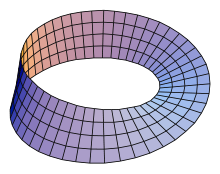
\includegraphics[scale = 0.5]{lec22_0.png}
\end{center}

\[\vec{r} = ((2 + u\cos v)\cos2v, \ (2 + u\cos v)\sin2v, \ u\cos v)\]
\[\vec{r}(0, \ v) = (2\cos v, 2\sin2v, 0) = \vec{r}(0, v + \pi)\]
\[\vec{N}(u, v) = (-4\sin v\cos2v, \ -4\sin v\sin2v, \ 4\cos v), \ \vec{N}(0, v) = -\vec{N}(0, v + \pi)\]\\
(Упражнение: вычислить $A, \ B, \ C$)
\section{Первая квадратичная форма поверхности}

Рассмотрим гладнкую и двухстороннюю поверхность $\vec{r} = \vec{r}(u, \ v) = (x(u, \ v), \ y(u, \ v), z(u, \ v))$\\

 \emph{Первой квадратичной формой поверхности} называют велечину : 
 \[I = (d\vec{r})^2 = <d\vec{r}, \ d\vec{r}> = <\vec{r'}_udu + \vec{r'}_vdv, \ \vec{r'}_udu + \vec{r'}_vdv> = <\vec{r'}_u, \ \vec{r'}_u>^2du^2 + 2<\vec{r'}_u, \ \vec{r'}_v>dudv + \] \[ + <\vec{r'}_v, \ \vec{r'}_v>^2dv^2 = Edu^2 + 2Fdudv + Gdv^2\]
 где $E, \ G, \ F$ ~--- \emph{коэффициенты квадратичной формы}.\\
\[E = <\vec{r'}_u, \ \vec{r'}_u>^2 = (x'_u)^2 + (y'_u)^2 + (z'_u)^2, \ 
F = x'_ux'_v + y'_uy'_v + z'_uz'_v, \ G = (x'_v)^2 + (y'_v)^2 + (z'_v)^2\]
Введена в употребление Гауссом в середине 19ого века.

\section{Вычисление длины кривой на поверхности}


   Пусть в области $D$ задана кривая 
$\lambda : \begin{cases}
             u = u(t),\\
             v = v(t),\\
             \alpha \leq t \leq \beta;
            \end{cases}$\\
Тогда $\vec{r}(u(t), \ v(t)) = \vec{\rho}(t) = (x(u(t), \ v(t)), \ y(u(t), \ v(t)), \ z(u(t), \ v(t)))$ задаёт некоторую кривую на поверхности, где $t$ пробегает отрезок $\left[\alpha, \ \beta\right]$.

Вычислим длинну кривой : 
\[
l = \int\limits_\alpha^\beta\sqrt{(x'_t)^2 + (y'_t)^2 + (z'_t)^2}dt = \int\limits_\alpha^\beta\sqrt{(dx)^2 + (dy)^2 + (dz)^2} = \int\limits_\alpha^\beta  |d\rho| =  \int\limits_\alpha^\beta|d\vec{r}| = \int\limits_\alpha^\beta\sqrt{(d\vec{r})^2} = \] 
\[ 
= \sqrt{Edu^2 + 2Fdudv + Gdv^2} \text{, где } u = u(t), \ v = v(t). 
\]
\textbf{Пример:}

На сфере радиуса $r = a$ задана кривая :
\[\begin{cases}
 x = a\cos u\cos v,\\
 y = a\cos u\sin v,\\
 z = a\sin u,
 \end{cases}
 -\frac{\pi}{2} \leq u \leq \frac{\pi}{2},
 0\leq t \leq 2\pi\]
\[\begin{cases}
u = t,\\
v = \ln\tg(\frac{\pi}{4} + \frac{t}{2});
\end{cases} \ 0 \leq t \leq 1\]
Найдём коэффициенты первой квадратичной формы. Для сферы $\vec{r} = (x(u, \ v), y(u, \ v), z(u, \ v))$
\[
\begin{cases}
z'_u = (-a\sin u\cos v, \ -a\sin u\sin v, \ a\cos v),\\
z'_v = (-a\cos u\sin v, \ a\cos u\cos v, \ 0);
\end{cases}
\]
\[
E = a^2, \ F = 0, \ G = a^2\cos^2u
\]
\[
\text{Тогда длинна кривой } l = \int\limits_0^1\sqrt{a^2d(u(t)^2) + a^2\cos^2u(t)d(v(t)^2)} =
\]
\[\int\limits_0^1\sqrt{a^2dt^2 + a^2\cos^2t(\frac{1}{\tg(\frac{\pi}{4} + \frac{t}{2})\cos^2(\frac{\pi}{4} + \frac{t}{2})})} = \int\limits_0^1\sqrt{a^2dt^2 + a^2dt^2} = a\sqrt{2}
\]
\section{Площадь поверхности}
Пусть задана гладкая двусторонняя поверхность $\pi : \vec{r} = \vec{r}(u, v), \ (u, v) \in D$.

\begin{center}
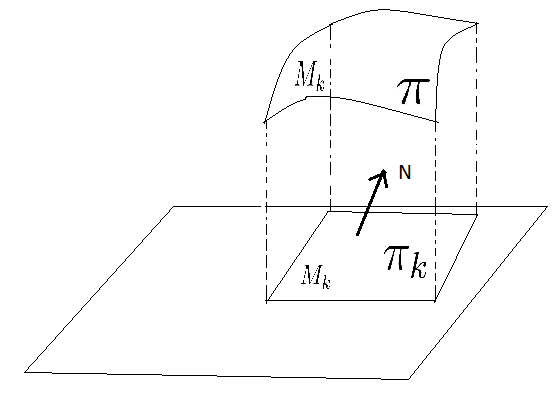
\includegraphics[scale = 1]{lec22_1.png}
\end{center}

Разобъём $\pi$ на части $\pi_k$. Выберем точку $M_k$ и построим касательную плоскость. Спроецируем $\pi_k$ на касательную плоскость. Получим некоторое множество $P_k$ с площадью $\Delta S_k$. Тогда площадь $\pi$ ~--- $S_\pi \approx \sum\Delta S_k$, то есть $S_\pi = \lim\limits_{\delta\rightarrow0}\sum\limits_{k = 1}^n\Delta S_k$, где $\delta$ ~--- диаметр разбиения.

\section{Вычисление площади}

Если поверхность гладкая и двусторонняя, то она имеет площадь, то есть квадрируема. В таких случаях не важно, каким будет разбиение на части $\pi_k$. Мы рассмотрим разбиение, построенное с помощью координатных прямых. Рассмотрим элемент площади, который соответствует $\vec{r} = \vec{r}(u, v), \ \vec{r} = \vec{r}(u + \Delta u, \ v), \ \vec{r} = \vec{r}(u, \ v + \Delta v)$.

\begin{center}
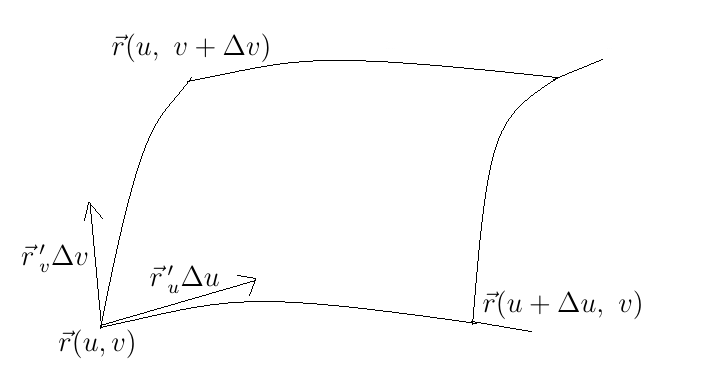
\includegraphics[scale = 1]{lec22_2.png}
\end{center}

Для достаточно мелкого разбиения площадь поверхности приближённо равна площади этого элемента. Тогда, $\Delta S_k \approx \left|[\vec{r'_u}\Delta u, \ \vec{r'_v}\Delta v\right]| = |\left[r'_u, \ r'_v\right]|\Delta u\Delta v$. Суммирую площади и переходя к пределу $S_\pi = \int\limits_D\int|\left[r'_u, \ r'_v\right]|dudv = \int\limits_D\int|\vec{N}|dudv = \int\limits_D\int\sqrt{A^2+B^2+C^2}dudv$

\[
(|\left[r'_u, \ r'_v\right]|)^2 = (\vec{z'_u})^2(\vec{z'_v})^2\sin\phi = EG(1 - \cos^2\phi) = EG - (|\vec{z'_u}||\vec{z'_v}|\cos\phi)^2 = EG-F^2\text{, т.~е.}
\]
\[
|\vec{N}| = \sqrt{EG - F^2}, \ S_\pi = \int\limits_D\int\sqrt{EG - F^2}
\]
\textbf{Пример:}\\
\[
\begin{cases}
 x = a\cos u\cos v, \\
 y = a\cos u\sin v,\\
 z = \sin u;
\end{cases} \ 
0 \leq u \leq 1, \ 0 \leq v \leq 1
\]
\[
 S_\pi = \int\limits_0^1du\int\limits_0^1\sqrt{EG-F^2} = \int\limits_0^1du\int\limits_0^1\sqrt{a^2\cos^2u}dv = a^2\int\limits_0^1du\int\limits_0^1\cos udv = a^2\sin\big|_0^1 = a^2\sin 1
\]
\section{Поверхностный интеграл первого рода}

Пусть дана двусторонняя гладкая поверхность $\pi$, $S$ ~--- её площадь. $\pi : \vec{r} = (x, \ y, \ z)$, на поверхности задана функция $f(x, \ y, \ z)$. Рассмотрим разбиение $\pi$ на кусочки $\pi_k, \ k = \overline{1, k}, \Delta S_k = S_{\pi_k}, \ \delta$ ~--- диаметр разбиения. На каждом кусочке $\pi_k$ возьмём любую точку $M_k \in \pi_k$ с координатами $M_k(x_k, \ y_k, \ z_k)$ и построим сумму $\sigma = \sum\limits_{k = 1}^nf(x_k, \ y_k, \ z_k)\Delta S_k$\\
$\lim\limits_{\delta\rightarrow0}\sigma = \int\limits_\pi\int f(x, \ y, \ z)ds$ ~--- \emph{поверхностный интеграл первого рода}(ПовИ-1).

\textbf{Физический смысл}
По поверхности $\pi$ распределяется масса с переменной плотностью $\rho = f(x, \ y, \ z)$, тогда величина $f(x_k, \ y_k, \ z_k)\Delta S_k$ ~--- это приблизительно $m_k$ ~--- масса кусочка $\pi_k$. Если просуммировать элементарные массы, то получим приближённую массу на поверхности, а переходя к пределу получим $m = \int\limits_\pi\int f(x, \ y, \ z)ds$
\end{document}

